
The dependency graph is notated as follows:
 %
{
   \[
     \progG(c) = (\progV(c), \progE(c), \progW(c), \progF(c))
     \]
 }
 with $\progV(c), \progE(c), \progW(c)$ and $ \progF(c)$ as computed in each steps above.
 % and $\progF(c) =\left\{(x^l, n)  \in  \mathcal{LV} \times \{0, 1\} 
 % ~ \middle\vert ~
 % x^l \in \lvar_{c},
 % n = 1 \iff x^l \in \qvar_{c} \land n = 0 \iff  x^l \in \qvar_{c} .
 % \right\} $,
 % This program-based graph program-based graph has a similar topology structure as 
 % % the one
 % % of 
 % the execution-based dependency graph. It has the same
 % vertices and query annotations, but approximated edges and weights.  
 % The algorithm computation is 
 Its formal definition can be found in the appendix.
 We compute the adaptivity upper bound for a program $c$ by the maximum query length over all finite walks in the program-based data dependency graph $\progG({c})$, defined  formally in Definition~\ref{def:prog_adapt}. 
 %
 We use $\walks(\progG(c))$ to represent the walks over the program-based dependency graph for $c$.
 Different from the walks on $\traceG(c)$, $k \in \walks(\progG(c))$ doesn't rely on the initial trace.
 The occurrence time of every $v_i $ in $k$'s vertices sequence is bound by 
 an arithmetic expression $w_i$ where $(v_i, w_i) \in \progW(c)$ is $v_i$'s estimated weight. Then we have $\qlen(k) \in \mathcal{A}_{in}$ as well. The full definition for $\walks(\progG(c))$ and $\qlen$ over $\walks(\progG(c))$ is in the appendix.
 %
 % The adaptivity upper bound 
 % is estimated as
 % Then the adaptivity bound based on program analysis for ${c}$ 
 % is the number of query vertices on a finite walk in $\progG({c})$. This finite walk satisfies:
 % \begin{itemize}
 % \item the number of query vertices on this walk is maximum
 % \item the visiting times of each vertex $v$ on this walk is bound by its reachability bound $\weights(v)$.
 % \end{itemize}
 
 % is computed as the maximum query length over all finite walks in $\walks(\progG({c}))$, and computed 
 
 %
 % It is formally defined in \ref{def:prog_adapt}.
 % defined formally as follows.
 %
 %
 \begin{defn}
 [{Program-Based Adaptivity}].
 \label{def:prog_adapt}
 \\
 {
 Given a program ${c}$ and its program-based graph 
 $\progG({c})$
 %  = (\vertxs, \edges, \weights, \qflag)$,
 %
 the program-based adaptivity for $c$ is 
 % a function $\progA({c}): \mathcal{T} \to\mathbb{N} $,
 % for an initial trace $\trace_0 \in \mathcal{T}$,
 defined as%
 \[
 \progA({c})
 \triangleq \max
 \left\{ \qlen(k) \ \mid \  k\in \walks(\progG({c}))\right \}.
 \]
 }
 \end{defn}
 Based on our soundness of the program-based adaptivity, our program-based adaptivity is a sound upper bound of its adaptivity in Definition~\ref{def:trace_adapt}. 
 \begin{thm}[Soundness of $\progA(c)$]
     \label{thm:sound_progadapt}
     For every program $c$, 
     % for any initial trace $\trace_0$, 
     its program-based adaptivity is a sound upper bound of its adaptivity.
      $$ \forall \trace_0 \in \mathcal{T}_{0}(c) \st 
 \config{\progA(c), \trace_0} \earrow n \implies n \geq A(c)(\trace_0) $$
 \end{thm}
 % By $\progA(c) \geq A(c)$, 
 % % between a function and an arithmetic expression,
 % we bound over all trace, $\forall \trace \in \mathcal{T} \st 
 % \config{\progA(c), \trace} \earrow n \implies n \geq A(c)(\trace) $.
 To estimate a sound and precise upper bound on adaptivity, we develop an adaptivity estimation algorithm called $\pathsearch$ (in the appendix Alg.~I), which uses both the deep first search and breath first search strategy to find the walk. We also show that the estimated adaptivity from our $\pathsearch$ is sound with respect to the program-based adaptivity. 
 \begin{thm}[Soundness of $\pathsearch$]
     \label{thm:sound_adaptalg}
     For every program $c$.
     % for any initial trace $\trace_0$,
      $$\pathsearch(\progG({c})) \geq \progA(c).$$
 \end{thm}
 The full proofs and details of all the soundness can be found in the appendix.
 
  The key novelty of AdaptSearch is its walk finding part, we first discuss two challenges when we try to find the walks in the program-based dependency graph, and show that how we solve them using our algorithms.
 
 % \paragraph*{Challenges}
 % Following is the challenge of computing the adaptivity on a program based dependency graph.
 % \\
 % In order to 
 % % search for the finite walk having the longest query length, which isn't a simple longest weighted path.
 % compute the adaptivity for a program $c$ on its estimated program-based dependency Graph $\progG(c)$, we need to 
 % search for the finite walk having the longest query length.
 % \\
 % % However, the finite walk isn't a simple weighted path by Definition~\ref{def:finitewalk}, there are two challenges in order to find this walk.
 % However, by Definition~\ref{def:finitewalk}, this finite walk isn't easy to find, below are the challenges in order to find this walk.
 % \\
 \textbf{Non-Termination Challenge:}
 % Moreover, b
 One naive walk finding method is to simply traverse on this program-based dependency graph by decreasing the weight of every node by one after every visit. However, this simple 
 traversing strategy leads to a non-termination dilemma for most programs we are interested in because the weight can be a symbolic expression. 
 % % because the weight is symbolic and simply traversing leads to non-termination.
 % It is difficult to tell when to terminate the recursion when the domain of this symbolic expression isn't finite, some the walk may also be infinite.
 % While, in most of our cases, the programs' program-based dependency Graphs are having symbolic weights with infinite domains on vertices.
 Look at the simple example in Figure~\ref{fig:alg_adaptsearch_simplewhile}, where $k$ is the input variable from domain $\mathbb{N}$.
 %  in Figure~\ref{} in Section~\ref{sec:overview},
 \begin{figure}
 \centering
 {
 \small
 \begin{subfigure}{.4\textwidth}
 \begin{centering}
 $ 
 \begin{array}{l}
   \kw{whileSim(k)} \triangleq \\
   \clabel{ \assign{j}{k} }^{0} ;
   \clabel{ \assign{x}{\query(\chi[0])} }^{1} ; \\
       \ewhile ~ \clabel{j > 0}^{2} ~ \edo ~ \\
       \Big(
        \clabel{\assign{x}{\query(\chi[x]) }}^{3}  ; 
       \clabel{\assign{j}{j-1}}^{4}       \Big)
   \end{array}
 $
 \caption{}
 \end{centering}
 \end{subfigure}
 \quad
   \begin{subfigure}{.45\textwidth}
   \begin{centering}
   \begin{tikzpicture}[scale=\textwidth/22cm,samples=200]
 \draw[] (0, 7) circle (0pt) node
 {\textbf{$x^1: {}^{1}_{1}$}};
 \draw[] (0, 4) circle (0pt) node
 {{ $x^3: {}^{k}_{1}$}};
 % Counter Variables
 \draw[] (10, 7) circle (0pt) node {{$j^2: {}^{1}_{0}$}};
 \draw[] (10, 4) circle (0pt) node {{ $j^4: {}^{k}_{0}$}};
 %
 % Value Dependency Edges:
 \draw[ ultra thick, -latex, densely dotted,] (0, 4.2)  -- (0, 6.5) ;
 \draw[ ultra thick, -Straight Barb, densely dotted,] (2, 4.5) arc (150:-180:1);
 \draw[ thick, -Straight Barb] (11.3, 4.7) arc (150:-150:1);
 \draw[ thick, -latex] (10, 4.6)  -- (10, 6.5) ;
 % Control Dependency
 \draw[ thick,-latex] (1.5, 7)  -- (8, 7) ;
 \draw[ thick,-latex] (1.5, 4)  -- (8, 7) ;
 \draw[ thick,-latex] (1.5, 7)  -- (8, 4) ;
 \draw[ thick,-latex] (1.5, 4)  -- (8, 4) ;
 \end{tikzpicture}
 \caption{}
   \end{centering}
   \end{subfigure}
 }
 % \end{wrapfigure}
 % \end{equation*}
 \vspace{-0.4cm}
  \caption{(a) The simple while loop example (b) The program-based dependency graph generated from $\THESYSTEM$.}
 \label{fig:alg_adaptsearch_simplewhile}
 \vspace{-0.5cm}
 \end{figure}
 % Analysis Results: $ \progA(\kw{whileRec}(k)) = 1 + k$
 %
 If we traverse on the program-based dependency graph, and decrease the weight of $x^3$ (the weight $k$ is symbolic) by one after every visit,
 % We can simply adopt either a deep first strategy to estimate the adaptivity as the length of the longest weight path, as 
 % in Alg.~\ref{alg:overadp_alg}.
 we will never terminate because we only know $k \in \mathbb{N}$.
 
 To solve this non-termination challenge, we switch to another walk finding approach: we first find a longest path in the program-based dependency graph and then approximate the walk with the path.
 Through a simple deep first search algorithm, we find the longest weighted path as the dotted arrow in Figure~\ref{fig:alg_adaptsearch_simplewhile},
 $x^3: {}^k_1 \to x^1: {}^1_1 $.
 Then, by summing up the weights on this path where the vertices have query annotation $1$, deep first search algorithm gives the adaptivity bound $1 + k$.
 This is a tight bound for this program's adaptivity. This approach is the fundamental of $\pathsearch$.
 % Look at the two-round example in overview, 
 % it is easy to find that the longest weighted path is  $x^3 : {}^{k}_{1} \to a^5 : {}^{k}_{0} \to l^6 : {}^{1}_{0}$ with weighted query length $1 + k$.
 % If we use this path to approximate a finite walk, and weight of each vertex as
 % %  their visiting times, 
 % its visiting time,
 % then it isn't a qualified walk. 
 % In the approximated walk, we have the vertices as $x^3 \to \cdots \to x^3 \to a^5 \to \cdots \to a^5 \to l^6$.
 
 % However, this gives us over-approximation to a large extend in other cases as in \textbf{Approximation Challenge}.
 % In Alg.~\ref{alg:adpt_alg}, 
 % we first find all the strong connected components of this graph, 
 \textbf{Approximation Challenge:}
 % As in Definition~\ref{def:finitewalk}, w
  We adopt a deep first strategy to search for the longest weighted path, and then use the path to approximate the adaptivity. We find that this gives us over-approximation to a large extend.
 % Specifically, according to the finite walk definition in Definition~\ref{def:finitewalk},
 % the visiting time of every vertex on a walk should be no more than its weight.
 % However, by searching for the longest weighted path, 
 % % and approximating the finite walk by this weight path, 
 % and use it as the approximated finite walk with the longest query length, 
 % the visiting times of the vertex on 
 % % it 
 % this approximated walk could 
 % % possibly 
 % exceed 
 % % its weights. 
 % the visiting times it can have.
 % Then, this approximated walk isn't a qualified walk by Definition~\ref{def:finitewalk}, 
 % and the weighted query length of this path is obviously greater than the maximum query length of the finite walk.
 This over-approximation could result in an $\infty$ adaptivity upper bound on the program with actual adaptivity $2$.
 Look at $\kw{twoRounds}$ in overview, 
 we find the longest weighted path is  $x^3 : {}^{k}_{1} \to a^5 : {}^{k}_{0} \to l^6 : {}^{1}_{0}$ in Figure~\ref{fig:overview-example}(c)  with weighted query length $1 + k$.
 If we use this path to approximate a finite walk, and weight of each vertex as
 %  their visiting times, 
 its visiting times,
 we have the estimated walk $x^3 \to \cdots \to x^3 \to a^5 \to \cdots \to a^5 \to l^6$, in which $x^3$ appears $k$ times. 
 Obviously,
 % the with the weighted length $1 + k$. It is obviously
 its weighted query length, $1 + k$, 
 % which is 
 over approximates 
 % its 
 the adaptivity of this example to a large extend, which is supposed to be $2$. 
 % \wq{
 % The reason of the over-approximation comes from the missing consideration of circle in the graph when we approximate the walk from a weighted path. 
 % If there is a circle in the graph, we can estimate in this way, but if there is no circle in our two round example, it is an over-estimation.
 % } 
 The reason of the over-approximation comes from the missing consideration of the restriction on vertex's visiting times in a walk.
 Moreover, the restriction plays different roles in cases
 whether there is cycle in the graph.
 % weights and cycles in the graph when we approximate the walk from a weighted path. 
 % It over-approximated the 
 % If there is a circle in the graph, we can estimate in this way, but if there is no circle in our two round example, it is an over-estimation.
 This leads us to consider cycle in the program-based dependency graph in $\pathsearch$, and we develop an auxiliary algorithm to estimate the adaptivity for cycles in the graph, $\kw{\pathsearch_{scc}(G)}$ as in Alg.~\ref{alg:adaptscc}.
 $\kw{\pathsearch_{scc}}$ takes an strong connected graph, which is an strong connected component (SCC) of $\progG(c)$
 % representing a cycle 
 and approximates the
 path to a precise walk to compute the adaptivity of this subgraph. 
 In general, $\pathsearch$ will now first find all the SCCs of $\progG(c)$ by using the Kosaraju’s algorithm\cite{sharirM81}.  
 Then $\pathsearch$ simplifies  the input graph by replacing every strong connected components with, a vertex whose weight is the adaptivity of the SCC, calculated by $\kw{\pathsearch_{scc}(G)}$. Then $\pathsearch$ performs
      the standard breath first search strategy to find the longest weighted path on this simplified graph and returns the estimation on adaptivity as we shown before.
      The full details of $\pathsearch$ is in the appendix Alg.~2.
 % The  as shown in appendix Alg.~I, takes our program-based dependency graph as input, and outputs the estimated adaptivity by two steps. 1. Process the input graph to a simplified graph 2. Perform
 %      the standard breath first search strategy to find the longest weighted path on this simplified graph and return the length as adaptivity.
 %     The step 2 is not interesting, we now discuss step 1. The input dependency graph may contain circle due to the while loop, we simplify (shrank) the input graph by replacing every strong connected components(circle) of the graph with, the vertex whose weight is the adaptivity of the SCC (a subgraph of the input one) calculated by our $\pathsearch$. The SCC is found by using the Kosaraju’s algorithm  \wq{cite}.  
 % % }
 %
 % \paragraph*{The Adaptivity Computation Algorithm ($\pathsearch$)}
 % \begin{algorithm}
 %     \caption{
 %     {Adaptivity Computation Algorithm ($\pathsearch$)}
 %     \label{alg:adpt_alg}
 %     }
 %     \begin{algorithmic}[1]
 %     \REQUIRE $G = (\vertxs, \edges, \weights, \qflag)$ \#\{The program based dependency graph\}
 %     % with a start vertex $s$ and destination vertex $t$ .
 %     \STATE  {\bf {$\kw{\pathsearch(G)}$}:}  
 %     \STATE {\bf init} 
 %     % \\
 %     % current node: $c$, 
 %     \\
 %     $q$: empty queue.
 %     % \\
 %     % $\kw{visited}$: List of length $|\vertxs|$, initialize with $\efalse$.
 %     % \\
 %     % $\kw{SSCvisited}$: List of length $|\vertxs|$, initialize with $\efalse$.
 %     % \\ 
 %     % $\kw{adapt_{scc}(SCC_i) = \pathsearch_{scc}(SCC_i)}$.
 %     \\
 %     $\kw{adapt}$ : the adaptivity of this graph initialize with $0$.
 %     \\
 %     \STATE Find all Strong Connected Components (SCC) in $G$: $\kw{SCC_1}, \cdots, \kw{SCC_n}, 0 \leq n \leq |\vertxs|$, 
 %     % where $\kw{SCC_i} = (\vertxs_i, \edges_i, \weights_i, \qflag_i)$.
 %     % and assign each vertex $x^i$ with an SCC number $\kw{SCC}(x^i)$
 %     \STATE {\bf for} every SCC: $\kw{SCC_i}$, compute its Adaptivity $\kw{SCC_i}$:
 %     \STATE \quad $\kw{adapt_{scc}[SCC_i] = \pathsearch_{scc}(SCC_i)}$;
 %     \STATE {\bf for} every $\kw{SCC_i}$:
 %     \STATE \qquad $q.append(\kw{SCC_i})$;
 %     \STATE \qquad $\kw{adapt_{tmp}} = 0$;
 %     \STATE \qquad {\bf while} $q$ isn't empty:
 %     \STATE \qquad \qquad $\kw{s} = q.pop()$;  \#\{take the top SCC from head of queue\}
 %     \STATE \qquad \qquad  $\kw{adapt_{tmp}}_0= \kw{adapt_{tmp}}$; \#\{record the adaptivity of last level\}
 %     \STATE \qquad \qquad  $\kw{SCC_{max}}$;  \#\{record the SCC with longest walk in this level\}
 %     % initialize cycle-adapt = 0.
 %     \STATE \qquad \qquad {\bf for} every 
 %     % SCC having a directed edge from $s$ of $s$: $\kw{SCC'}$:
 %     % directed edge goes out of $\kw{s}$ and connects a 
 %     different SCC, $\kw{s'}$ connected by $\kw{s}$ by a directed edge from $\kw{s}$:
 %     % \STATE \qquad \qquad   cycle-adapt$ = \max($cycle-adapt, $\kw{dfs_{refine}(G, v, v)})$;
 %     % \STATE \qquad \qquad \qquad \#\{compute the adaptivity of vertex $v$  on $\kw{SCC}(v)$, and update r[v] with the SCC-adapt\}
 %     % \STATE \qquad \qquad \qquad $ r[v] = r[s] + \kw{dfs_{refine}(G, v, visited)})$; 
 %     \STATE \qquad \qquad \qquad {\bf if} $(\kw{adapt_{tmp}} < \kw{adapt_{tmp}}_0 + \kw{adapt_{scc}[s']})$:
 %     \STATE \qquad \qquad \qquad \qquad $\kw{adapt_{tmp}} = \kw{adapt_{tmp}}_0 + \kw{adapt_{scc}[s']}$; 
 %     \STATE \qquad \qquad \qquad \qquad $\kw{SCC_{max} = s'} $; \#\{update the SCC with longest walk in this level\} 
 %     % \STATE \qquad   $r[c] = r[c] + $cycle-adapt;
 %     % \STATE \qquad for all unvisited vertex $v$ having directed edge from c and $! \kw{cycle}(c)$:
 %     % \STATE \qquad \qquad $r[v] = r[c] + \flag(v)$; 
 %     % \STATE \qquad \qquad \qquad  \#\{mark all the nodes with the same $\kw{SCC}$ number as visited\} 
 %     % \STATE \qquad \qquad \qquad  \#\{append the unvisited vertex to the rear of the queue\}
 %     % \STATE \qquad \qquad \qquad  \#\{mark all the nodes with the same $\kw{SCC}$ number as visited\} 
 %     % \STATE \qquad \qquad for $v \in V$,   $\kw{visited}[s] = 1$;
 %     \STATE \qquad \qquad \qquad $q.append(\kw{SCC_{max}})$;
 %     \STATE \qquad $\kw{adapt} = \max(\kw{adapt}, \kw{adapt_{tmp}})$;    
 %     \RETURN $\kw{adapt}$.
 %     \end{algorithmic}
 %     \end{algorithm}
     %
 %
     % In Alg.~\ref{alg:adpt_alg}, 
     % it 
     % This algorithm first finds all the strong connected components (SCC) of $\progG(c)$ using the Kosaraju’s algorithm in line:3. 
     % Every $\kw{SCC_1}, \cdots, \kw{SCC_n}$
     % where $0 \leq n \leq |\vertxs|$ is a sub-graph of $\progG(c)$, where $\kw{SCC_i} = (\vertxs_i, \edges_i, \weights_i, \qflag_i)$.
     % % where $\kw{SCC_i} = (\vertxs_i, \edges_i, \weights_i, \qflag_i)$.
     % Then, 
     % % we compute the adaptivity on every SCC, which is a subgraph of the $\progG(c)$, in line:4-5 by Alg.~\ref{alg:adaptscc}.
     % it computes the adaptivity on every SCC
     % % , which is a subgraph of the $\progG(c)$, 
     % in line:4-5 by Alg.~\ref{alg:adaptscc}.
     % % We guarantee the soundness of the adaptivity on SCC by Lemma~\ref{lem:sound_adaptalg_scc} with proof 
     % in appendix.
     % % ~\ref{apdx:adaptalg_soundness}.
     % The $\progG(c)$ is then shrunk into an acyclic directed graph where 
     % % vertices are all the SCCs and edges are between every SCCs with their adaptivities as weights.
     % $\kw{SCC_1}, \cdots, \kw{SCC_n}$ are vertices with their adaptivities as weights.
     % % , and directed edges are .
     % For every $(v_i, v_j) \in \edges$ such that $v_1 \in \vertxs_i$, $v_j \in \vertxs_j$ and $i \neq j$,
     % there is a edge $(s_i, s_j)$ in this shrank graph. \\ 
     % Then, we use the standard breath first search strategy to find the longest weighted path
     % %  w.r.t. all the SCCs and their adaptivities.
     % on this shrank graph and return the length as adaptivity.
     % \\
     % We guarantee that 
     % % this longest weighted path is a sound computation of the adaptivity on this,
     % the length of this longest weighted path is a sound computation of the adaptivity for program $c$,
     % % as well as 
     % and this longest weighted path a sound computation of the finite walk having the longest query length 
     % % on this graph, in Theorem~\ref{thm:sound_adaptalg}
     % on $c$'s program based dependency graph, in Theorem~\ref{thm:sound_adaptalg}
     % in appendix.
     % ~\ref{apdx:adaptalg_soundness}.
 %    
 % \todo{add proof} 
 % We also guarantee the conditional completeness of the adaptivity computation for graphs under the case that 
 % $c$'s program-based dependency Graph $\progG(c)$ is acyclic directed
 % % in Theorem~\ref{thm:adaptalg_pcomplete} 
 % in appendix.
 
 % ~\ref{apdx:adaptalg_completeness}.
     % for every vertex which isn't on any SCC, it is easy to know that it will be visited 
     % at most once given no edges going back to this vertex. We can know the adaptivity on the SCC 
      %
     % \begin{algorithm}
     % \caption{
     % {Longest Adaptivity Search Algorithm ($\pathsearch$)}
     % \label{alg:adpt_alg}
     % }
     % \begin{algorithmic}
     % \REQUIRE Weighted Directed Graph $G = (\vertxs, \edges, \weights, \flag)$ with a start vertex $s$ and destination vertex $t$ .
     % \STATE  {\bf {bfs $(G)$}:}  
     % \STATE {\bf init} 
     % \\
     % current node: $c$, 
     % \\
     % queue: $q$ : List, add into $a$ an arbitrary v from $\vertxs$. 
     % \\
     % visited: List of length $|\vertxs|$, initialize with $\efalse$.
     % \\
     % results: $r$ : List of length $|\vertxs|$, initialize with -1.
     % \\
     % curr$\kw{flowcapacity}$: INT, initialize MAXINT.
     % \\
     % querynum: INT, initialize 0. \#\{To count the query numbers when we are walking inside a cycle\}
     % \\
     % \STATE \qquad {\bf while} $q$ isn't empty:
     % \STATE \qquad \qquad take the vertex from head $c= q.pop()$
     % \STATE \qquad \qquad mark $c$ as visited, visited $[c] = 1$.
     % \STATE \qquad \qquad {\bf if} $\kw{cycle}(c)$  \#\{we are inside a cycle\}
     % \STATE \qquad \qquad \qquad curr$\kw{flowcapacity}$ = min($\weights$(c), curr$\kw{flowcapacity}$).
     % \STATE \qquad \qquad \qquad querynum += $\flag(c)$.
     % \STATE \qquad \qquad  \qquad for all unvisited vertex $v$ having directed edge from c:
     % \STATE \qquad \qquad \qquad \qquad r[v] = r[c]; q.add(v)
     % \STATE \qquad \qquad \qquad  {\bf if}  $v$ is visited, then the circle finished
     % \STATE \qquad \qquad \qquad \qquad update the result $r[v] =  \max(r[v], r[c] + $curr$\kw{flowcapacity}$*querynum)
     % \STATE \qquad \qquad \qquad \qquad curr$\kw{flowcapacity}$ = MAXINT
     % \STATE \qquad \qquad \qquad \qquad querynum = 0.  
     % \STATE \qquad \qquad {\bf else} 
     % \STATE \qquad \qquad \qquad for all unvisited vertex $v$ having directed edge from c:
     % \STATE \qquad \qquad \qquad  \qquad $r[v] = \max(r[v], r[c] + \flag(c))$; q.add(v)
     % \RETURN max($r$)
     % \end{algorithmic}
     % \end{algorithm}
     %
     % \begin{algorithm}
     %   \caption{
     %   {Over-Approximated Adaptivity on SCC}
     %   \label{alg:overadp_alg}
     %   }
     %   \begin{algorithmic}[1]
     %   \REQUIRE $G = (\vertxs, \edges, \weights, \qflag)$ \#\{An Strong Connected Symbolic Weighted Directed Graph\}
     %   % with a start vertex $s$ and destination vertex $t$ .
     %   \STATE {\bf {$\kw{\pathsearch_{scc-naive}(G)}$}:}  
     %   \STATE {\bf init} 
     %   \\
     %   $\kw{r_{scc}}$: the Adaptivity of this SCC
     %   % \STATE  {\bf def} {$\kw{dfs_{naive}(G, c,visited)}$}: 
     %   % % \STATE {\bf init} 
     %   % % \\
     %   % % current node: $c$, 
     %   % % \\
     %   % % visited: List of length $|\vertxs|$, initialize with $\efalse$.
     %   % % \\
     %   % % \STATE {\bf if} $c = s$:
     %   % % \RETURN \qquad  $\weights(s)*\flag(s) $.
     %   % \STATE \qquad $r[c] = \weights(c)*\qflag(c) $
     %   % \STATE \qquad {\bf for}  all vertex $v$ having directed edge from $c$:
     %   % \STATE \qquad \qquad {\bf if}  $v$ is unvisited:
     %   % \STATE \qquad \qquad \qquad  \#\{mark $v$ as visited\} $\kw{visited}[v] = 1$;
     %   % \STATE \qquad \qquad \qquad $r[c] += \kw{dfs_{naive}(G, v, visited)}$;
     %   % \STATE \qquad {\bf else}: \#\{There is a cycle finished\}
     %   % \RETURN \qquad \qquad $\weights(v)*\flag(v) $.
     %   \STATE  {\bf for} every vertex $v$ in $\vertxs$:
     %   % \STATE  \qquad initialize \kw{visited} with $\efalse$.
     %   \STATE  \qquad $r_{scc} += \weights(v)*\qflag(v)$  
     %   \RETURN $r[c]$
     %   \end{algorithmic}
     %   \end{algorithm}
       %
 %
     % \begin{algorithm}
     %     \caption{
     %     {Over-Approximated Adaptivity on SCC}
     %     \label{alg:overadp_alg}
     %     }
     %     \begin{algorithmic}
     %     \REQUIRE Weighted Directed Graph $G = (\vertxs, \edges, \weights, \qflag)$ with a start vertex $s$ and destination vertex $t$ .
     %     \STATE  {\bf {$\kw{dfs_{naive}(G, c,visited)}$}:}  
     %     % \STATE {\bf init} 
     %     % \\
     %     % current node: $c$, 
     %     % \\
     %     % visited: List of length $|\vertxs|$, initialize with $\efalse$.
     %     % \\
     %     % \STATE {\bf if} $c = s$:
     %     % \RETURN \qquad  $\weights(s)*\flag(s) $.
     %     \STATE $r[c] = \weights(c)*\qflag(c) $
     %     \STATE {\bf for}  all vertex $v$ having directed edge from $c$:
     %     \STATE \qquad {\bf if}  $v$ is unvisited:
     %     \STATE \qquad \qquad  \#\{mark $v$ as visited\} $\kw{visited}[v] = 1$;
     %     \STATE \qquad \qquad $r[c] += \kw{dfs_{naive}(G, v, visited)}$;
     %     % \STATE \qquad {\bf else}: \#\{There is a cycle finished\}
     %     % \RETURN \qquad \qquad $\weights(v)*\flag(v) $.
     %     \RETURN $r[c]$
     %     \end{algorithmic}
     %     \end{algorithm}%
         %
   \paragraph*{Adaptivity Computation Algorithm on SCC Graph ($\kw{\pathsearch_{scc}(G)}$)}
     \begin{algorithm}
             \caption{
             {Adaptivity Computation Algorithm on SCC Graph  {\bf {$\kw{\pathsearch_{scc}(G)}$}:} }
             \label{alg:adaptscc}
             }
             \begin{algorithmic}[1]
               \REQUIRE $G = (\vertxs, \edges, \weights, \qflag)$ \#\{An Strong Connected program based dependency Graph\}
             % \STATE  {\bf {$\kw{\pathsearch_{scc}(G)}$}:}  
             \STATE {\bf init} 
             % \\
             $\kw{r_{scc}}$: $\aexpr$, arithmetic expression, initialized $0$, the Adaptivity of this SCC
             % \STATE \qquad {\bf init} 
             % \STATE \qquad current node: $c$, 
             % \\
             % visited: List of length $|\vertxs|$, initialize with $\efalse$.
             % \\ \qquad  $\kw{r_{scc}}$ : initialize $0$, the adaptivity of this graph
             \\ \qquad  $\kw{visited}$ : $\{0, 1\}$ List,  \#\{length $|\vertxs|$, initialize with $0$ for every vertex\}
             % \\ \qquad  \#\{length $|\vertxs|$, initialize with $0$ for every vertex, recording whether a vertex is visted.\}
             \\ \qquad  $\kw{r}$ : $\aexpr$, arithmetic expression List, 
             \#\{length $|\vertxs|$, initialize with $\qflag(v)$ for every vertex \}
             % \\ \qquad  \#\{length $|\vertxs|$, initialize with $\qflag(v)$ for every vertex, recording the adaptivity reaching each vertex.\}
             \\ \qquad  $\kw{flowcapacity}$: $\aexpr$ List, 
             \#\{length $|\vertxs|$, initialize with $\infty$ for every vertex\}
             % INT List of length $|\vertxs|$, initialize MAXINT. 
             % \\ \qquad  \#\{length $|\vertxs|$, initialize with $\infty$ for every vertex,
             % % \#\{For every vertex, 
             % recording the minimum weight when the walk reaching 
             % that vertex, inside a cycle\}
             \\ \qquad  $\kw{querynum}$: INT List,  \#\{length $|\vertxs|$, initialize with $\qflag(v)$ for every vertex.
             % % \#\{For every vertex, 
             % recording the query numbers when the path reaching 
             % that vertex, inside a cycle
             \}
             % %  of length $|\vertxs|$, initialize with $\qflag(v)$ for every vertex. 
             % \\ \qquad  \#\{length $|\vertxs|$, initialize with $\qflag(v)$ for every vertex, 
             % \#\{For every vertex, 
             % recording the query numbers when the path reaching 
             % that vertex, inside a cycle\}
             \STATE {\bf if} $|\vertxs| = 1$ and $|\edges| = 0$: {\bf return}  $\qflag(v)$
             % \STATE \qquad {\bf return}  $\qflag(v)$
             \STATE  {\bf def} {$\kw{dfs(G, c,visited)}$}:
             % \STATE \qquad update the length of the longest path reaching this vertex
             % $r[s] =  r[s] + $$\kw{flowcapacity}$[s] * querynum[s].
             % \RETURN  \qquad $r[s]$.      
             \STATE \qquad {\bf for} every vertex $v$ 
             % having directed edge from $c$:
             connected by a directed edge from $c$:
             \STATE \qquad \qquad {\bf if} $\kw{visited}[v] = \efalse$:
             \STATE \qquad \qquad \quad $\kw{flowcapacity[v] = \min(\weights(v), {flowcapacity}[c])}$;
             \STATE \qquad \qquad \quad $\kw{querynum[v] = querynum[c] + \qflag(v)}$;
             % \STATE \qquad \qquad \qquad \#\{do not update the length of the longest walk reaching $v$ until the cycle is finished\}
             % \STATE \qquad \qquad \qquad $\kw{r[v] =  r[c] + flowcapacity[v] \times querynum[v]} $; \#\{do not update the length of the longest walk reaching $v$ until the cycle is finished\}
             \STATE \qquad \qquad \quad $\kw{r[v] =  \max(r[v], flowcapacity[v] \times querynum[v]}) $; 
             % \#\{do not update the length of the longest walk reaching $v$ until the cycle is finished\}
             \STATE \qquad \qquad \quad  $\kw{visited}[v] = 1$;
             $\kw{dfs(G, v, visited)}$; %\#\{mark $v$ as visited\}
             % \STATE \qquad \qquad \qquad $\kw{dfs(G, v, visited)}$;
             \STATE \qquad \quad {\bf else}: \#\{There is a cycle finished, update the adaptivity\}
             % \STATE \qquad \qquad \qquad \#\{update the length of the longest path reaching this vertex\}
             \STATE \qquad \qquad \quad 
             $\kw{r[v] =  \max(r[v], r[c] +  \min(\weights(v), {flowcapacity}[c]) * (querynum[c] + \qflag(v)))}$;
             % \#\{update the length of the longest walk reaching this vertex on this cycle\}
             %  $\kw{r[v] =  \max(r[v], r[c] + flowcapacity[v] * querynum[v])}$; \#\{update the length of the longest walk reaching this vertex on this cycle\}
             %  \STATE \qquad \qquad \qquad \#\{Recover the $\kw{flowcapacity}$ and querynumber to previous state, for different loops\}
             % \STATE \qquad \qquad \qquad $\kw{flowcapacity[v] = flowcapacity[c]}$; \#\{Recover the $\kw{flowcapacity}$\}
             % \STATE \qquad \qquad \qquad $\kw{querynum[v] = querynum[c]}$;\#\{Recover the $\kw{querynum}$\}
             \STATE \qquad {\bf return}  $\kw{r[c]}$
             \STATE  {\bf for} every vertex $v$ in $\vertxs$:
             initialize the $\kw{visited, r, flowcapacity, querynum}$;
             % \STATE  \qquad initialize the $\kw{visited, r, flowcapacity, querynum}$;
             \STATE  \qquad $\kw{r_{scc} = \max(r_{scc}, dfs(G, v, \kw{visited} ))}$ ; 
             \RETURN  $\kw{r_{scc}}$
             \end{algorithmic}
             \end{algorithm}
             % \\
 % Following is the challenge of computing the adaptivity on a program based dependency graph.
 % In order to search for the finite walk having the longest query length, which isn't a simple longest weighted path.
 % \\
 % the visiting times of every vertex on this walk should be no more than its weight, which is a symbolic expression.
 % So we cannot simply search for the longest weight path where the visiting times of the vertex on it could possibly exceed its weights.
 % We can neither simply traverse on this graph by decreasing the weight of every node by 1 after every visiting,
 % because the weight is symbolic and simply traversing leads to non-termination.
 % \\
 % In Alg.~\ref{alg:adaptscc}, 
 
 
 This algorithm in Alg.~\ref{alg:adaptscc} takes a subgraph of the program-based dependency graph(SCC), and the output is the adaptivity of the input. 
 For an SCC containing only one vertex, it returns the query annotation of this vertex as adaptivity.
 For SCC containing at least one edge, 
 There are three steps: 1. find out all the paths in the input 2. calculate the adaptivity of every path using our designed adaptivity counting method. 3. return the maximal adaptivity among all the paths. Because our input graph is SCC, when we start traversing from a vertex, we will finally go back to this vertex. The paths we find in step 1 are all those with the same starting and ending vertex. The most interesting part is step 2. 
 % \wq{Add more about step 2 here, what it is and why it is good.}
 % Again, for 
 % the SCC containing only one vertex without any edge, as in line:4-5 in Alg.~\ref{alg:adaptscc}.
 % % then 
 % % If yes, then i
 % % it's easy to know that it will be visited 
 % % at most once since there isn't edge going back to this vertex. 
 % % So we can know 
 % The adaptivity on this SCC is at most one if it is a query vertex,
 % and zero otherwise.
 % $\kw{\pathsearch_{scc}(G)}$ return query annotation directly as in line:4-5.
 % % So $\kw{\pathsearch_{scc}(G)}$ return query annotation directly as in line:4-5.
 % \\
 % If not, then the 
 For the SCC containing at least one edge, 
 we compute the adaptivity for each path 
 on the fly of searching for the paths 
 in the
 % design a 
 recursion algorithm $\kw{dfs}$. It is designed based on 
 a deep first search strategy 
 % of this algorithm is described as follows,
 from line: 6-16.
 % searching for the paths 
 % starting from every vertex as step 1. 
 % In the meantime, it computes the adaptivity for each path during the path searching procedure, which is the step 2.
 % with special parameter 
 % searching for the finite walk having the longest query length
 % we are searching for the finite walk having the longest query length through a deep first search strategy.
 % The difficulty is, the visiting times of every vertex on this walk should be no more than its weight, which is a symbolic expression.
 % As the two challenges discussed above, 
 % we want to guarantee the visiting time of each vertex smaller than 
 % its weight and compute the adaptivity accurately, in the meantime guarantee the algorithm termination. 
 % It use a capacity limitation and  special parameters to achieve it,
 % specifically as follows.
 % Additionally, we are computing the query length rather than sum of the weights.
 % We design a deep first search strategy
 % % of this algorithm is described as follows,
 % from line: 6-16 in Alg.~\ref{alg:adaptscc}, 
 % searching for the finite walk having the longest query length
 %  through a deep first search strategy
 % with a capacity limitation and use special parameter to compute the adaptivity.
 % for every path.
 % So we cannot simply search for the longest weight path where the visiting times of the vertex on it could possibly exceed its weights.
 % We can neither simply traverse on this graph by decreasing the weight of every node by 1 after every visiting,
 % because the weight is symbolic and simply traversing leads to non-termination.
 % \\
 % We will explain some interesting part of the algorithm, which is related to solving the challenges.
 % In order to
 % guarantee the termination, 
 % % this algorithm 
 % $\kw{\pathsearch_{scc}(G)}$
 % terminates the recursion if monitored a cycle, as in line:8 and line:14, through a $\{0, 1\}$ list $\kw{visited}$.
 % This 
 % % guaranteed the termination and 
 % solved the \textbf{Non-Termination Challenge}.
 % \todo{solve the challenge 2} 
 % search for finite walk  
 % So we use the dfs to search for the 
 % \\
 In order to guarantee the visiting times of each vertex by its weight
 and compute the adaptivity accurately, 
 we use a special parameter $\kw{flowcapacity}$  to track the minimum weight
 along the path during the 
 % dfs process, 
 % deep first 
 searching procedure, 
 and a parameter $\kw{querynum}$
 % to compute the query length of this walk
 to track the total number of vertices with query annotation $1$
 % which are query vertices 
 along the path.
 % 
 % \todo{solve the challenge 1, specifically in the dfs strategy
 % of this algorithm is described as follows,
 % from line: 6-16 in Alg.~\ref{alg:adaptscc}. } 
 % \\
 % Then, to compute the query length of this walk, 
 % we use another parameter $\kw{querynum}$
 % to track the total number of vertices which are query vertices along the walk.
 
 % The detail steps of this dfs strategy
 % % of this algorithm is described as follows,
 % from line: 3-16 in Alg.~\ref{alg:adaptscc},
 % particularly from line: 7-15 on how to 
 % use these two special parameters to resolve \textbf{Challenge I}
 %  is described as follows.
 % searching for the finite walk having the longest query length through a deep first search strategy
 % with a capacity limitation and use special parameter to compute the adaptivity
 % for every path.
 % \\
 % We first initialize some parameters:
 % \\
 % $\kw{visited}$ is initialized as a list of $0$ for every vertex on this SCC, in order to guarantee the termination;
 % \\ 
 % $\kw{r}$ is initialized  as a list of integer with length $|\vertxs|$, initialize with $\qflag(v)$ for every vertex. The adaptivity reaching each vertex.
 % \\ 
 $\kw{flowcapacity}$ is a list of arithmeitc expression $\mathcal{A}_{in}$ 
 % for every vertex,
 recording the minimum weight when the path reaches that vertex, which is initialized by $\infty$.
 % , inside a cycle\}
 
 $\kw{querynum}$ is a list of integer
 % of all the vertices, which is 
 initialized by query annotation $\qflag(v)$ for every vertex. 
 % For every vertex, 
 % % recording the query numbers when the path reaching.
 % % in order to 
 % it records the total query numbers when the path reaching this vertex.
 
 % We maintain the minimum weight for the 
 % $\kw{flowcapacity}$, 
 % number of query vertices 
 % $\kw{querynum}$ 
 % and update the adaptivity for this path $\kw{r}$
 % alone the path and update the adaptivity reaching 
 % this vertex, 
 % when traversing on this graph, as in Alg.~\ref{alg:adaptscc} from line: 8-13.
 % % and then recursively dfs on all vertices heading out from this vertex.
 % % \\
 % At line: 15 where this vertex is visited, i.e., this path 
 % going back to its starting node,
 % we only update the adaptivity $\kw{r}$ reaching this vertex.
 % and neither recursion nor update the $\kw{flowcapacity}$  and 
 % $\kw{querynum}$.
 
 % Again, Non-recursion in the second branch
 % % in order to 
 % guarantees the termination and resolves \textbf{Non-Termination Challenge}.
 % \\
 The updating operations
 during the traverse 
 (line: 8) and 
 at the end of the traverse (line: 11) are interesting,
 % in these two branches, 
 specifically $\kw{flowcapacity[v] \times querynum[v]}$ 
 % in line: 11 and line: 15 
 computes the query length for this path. 
 it guarantees 
 the visiting times of each vertex on the path reaching a vertex $v$ is no more than 
 the maximum visiting times it can be on a qualified walk, through $\kw{flowcapacity[v]}$,
 and in the same time  compute the query length instead of weighted length accurately through 
 $\kw{ querynum[v]}$.
 %  its minimum visiting time, 
 In this way, we resolve the \textbf{Approximation Challenge} without losing the soundness, formally in the appendix.
 % ~\ref{apdx:adaptalg_soundness}.
 % this 
 % 2. then 
 % by using $\kw{flowcapacity[v] \times querynum[v]}$ to compute the query length. 
 % without lose the adaptivity.
 %
 
 Now, we show an example illustrating how our two updating operations for adaptivity 
 for each path can guarantee both the accuracy and the soundness. 
 % Notice here, another special operation we have in the second branch is Non-updating of
 % % Non-updating the 
 % $\kw{querynum}$ and $\kw{flowcapacity}$.
 % This guarantees both the accuracy and the soundness.
 % Specifically,
 % % because a second visiting of the same vertex 
 % if this vertex is visited, it indicates that a cycle is monitored and  
 % % indicates there is a cycle goes back to this vertex, 
 % the traversing on this cycle is finished by going back to this vertex.
 % %
 % % then, when 
 % When we continuously search for walks heading out of this vertex, 
 % the minimum weight on this cycle does not affect the walks going out of this vertex that not pass this cycle.
 % However, if we keep recording the minimum weight, then we
 % %  are restricting 
 % restrict the visiting times of vertices on a walk by
 %  using the minimum weight of vertices not on this walk.
 % %  , it is unsound anymore.
 % Then, it is obviously that this leads to unsoundness.
 % \todo{example} 
 % To under stand how the two operations 
 Look at a Nested While Loop example program in Figure~\ref{fig:alg_adaptsearch_nestedwhile}.
  %
   %
   \begin{figure}
     \centering
     {\small
     \begin{subfigure}{.5\textwidth}
     \begin{centering}
     % 
     $ 
     \begin{array}{l}
       \kw{nestedWhileMultiVarRecAcross}(k) \triangleq \\
       \clabel{\assign{i}{k} }^{0} ; 
       \clabel{ \assign{x}{\query(\chi[0])}}^{1} ; 
       \clabel{ \assign{y}{\query(\chi[1])}}^{2} ; \\
           \ewhile ~ \clabel{i > 0}^{3} ~ \edo ~ \\
           \Big(
            \clabel{\assign{i}{i-1}}^{4} ;
            \clabel{\assign{j}{k}}^{5} ;
            \clabel{\assign{y}{\query(\chi(\ln(x) + y))} }^{6}  ; \\
            \ewhile ~ \clabel{j > 0}^{7} ~ \edo ~ \\
            \Big(
             \clabel{\assign{j}{j-1}}^{8};
             \clabel{\assign{x}{\query(\chi(\ln(y))+\chi[x])} }^{9}
             \Big) \Big)
       \end{array}
     %       
     $
     \caption{}
     \end{centering}
     \end{subfigure}
     \quad
     \begin{subfigure}{.3\textwidth}
       \begin{centering}
       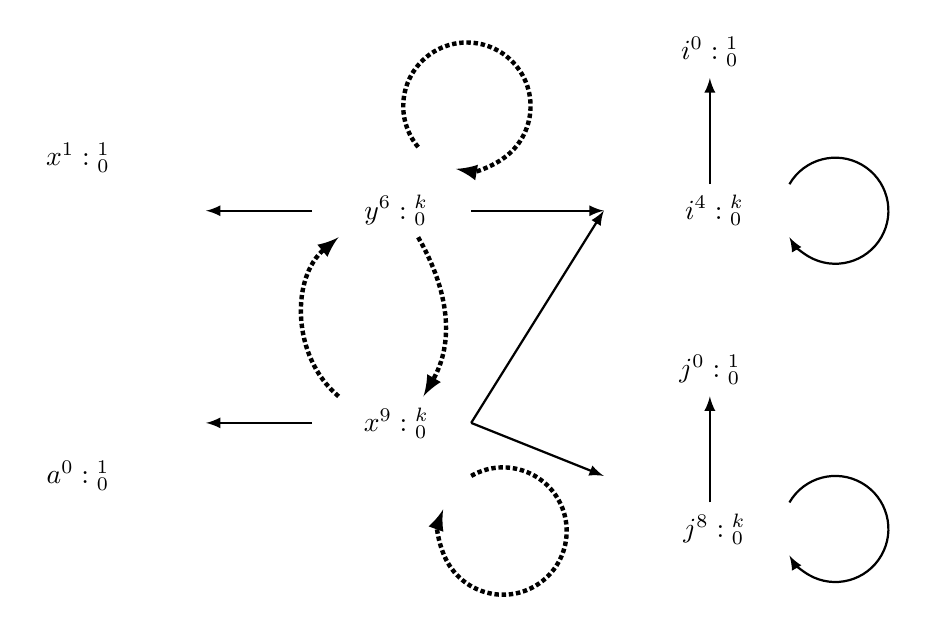
\begin{tikzpicture}[scale=\textwidth/18cm,samples=200]
 % Variables Initialization
 \draw[] (-6, 1) circle (0pt) node{{ $a^0: {}^1_{0}$}};
 \draw[] (-6, 7) circle (0pt) node{{ $x^1: {}^{1}_{0}$}};
 % Variables Inside the Loop
    \draw[] (0, 6) circle (0pt) node{{ $y^6: {}^{k}_{0}$}};
    \draw[] (0, 2) circle (0pt) node{{ $x^9: {}^{k}_{0}$}};
    % Counter Variables
    \draw[] (6, 9) circle (0pt) node {{$i^0: {}^{1}_{0}$}};
    \draw[] (6, 6) circle (0pt) node {{ $i^4: {}^{k}_{0}$}};
    \draw[] (6, 3) circle (0pt) node {{$j^0: {}^{1}_{0}$}};
    \draw[] (6, 0) circle (0pt) node {{ $j^8: {}^{k}_{0}$}};
    %
    % Value Dependency Edges:
    \draw[ ultra thick, -latex, densely dotted,] (0.5, 7.2) arc (220:-100:1.2);
    \draw[ thick, -latex] (6, 6.5)  -- (6, 8.5) ;
    \draw[ thick, -latex] (6, 0.5)  -- (6, 2.5) ;
    \draw[ ultra thick, -latex, densely dotted,] (1.5, 1.0) arc (120:-200:1.2);
    % Value Dependency Edges on Initial Values:
    \draw[ thick, -latex,] (-1.5, 2)  -- (-3.5, 2) ;
    \draw[ thick, -latex,] (-1.5, 6)  -- (-3.5, 6) ;
    %
    \draw[ ultra thick, -latex, densely dotted,] (-1, 2.5)  to  [out=-220,in=220]  (-1, 5.5);
    \draw[ ultra thick, -latex, densely dotted,]  (0.5, 5.5) to  [out=-60,in=60] (0.6, 2.5) ;
    % Control Dependency
   %  \draw[ thick,-latex] (1.5, 7)  -- (4, 9) ;
   %  \draw[ thick,-latex] (1.5, 4)  -- (4, 9) ;
   \draw[ thick, -latex, ] (7.5, 6.5) arc (150:-150:1);
   \draw[ thick, -latex, ] (7.5, 0.5) arc (150:-150:1);
   \draw[ thick,-latex] (1.5, 6)  -- (4, 6) ;
    \draw[ thick,-latex] (1.5, 2)  -- (4, 6) ;
    \draw[ thick,-latex] (1.5, 2)  -- (4, 1) ;
    \end{tikzpicture}
    \caption{}
       \end{centering}
       \end{subfigure}
     }
     % \end{wrapfigure}
     % \end{equation*}
     \vspace{-0.4cm}
      \caption{(a) The nested while loop example, (b) The program-based dependency graph generated from $\THESYSTEM$.}
     \label{fig:alg_adaptsearch_nestedwhile}
     \vspace{-0.7cm}
     \end{figure}
     %
     We first search for a path: $y^6 \to y^6$, and compute the adaptivity for this path as 
     $k$.
     Notice here, another special operation we have in the second branch is Non-updating of
 % Non-updating the 
 $\kw{querynum}$ and $\kw{flowcapacity}$.
 This guarantees both the accuracy and the soundness.
 Specifically,
 % because a second visiting of the same vertex 
 if this vertex is visited, it indicates that a cycle is monitored and  
 % indicates there is a cycle goes back to this vertex, 
 the traversing on this cycle is finished by going back to this vertex.
 %
 % then, when 
 When we continuously search for walks heading out of this vertex, 
 the minimum weight on this cycle does not affect the walks going out of this vertex that will not pass this cycle.
 However, if we keep recording the minimum weight, then we
 %  are restricting 
 restrict the visiting times of vertices on a walk by
  using the minimum weight of vertices not on this walk.
 %  , it is unsound anymore.
 Then, it is obviously that this leads to unsoundness.
   If we update the $\kw{flowcapacity}[y^6]$ as $k$ after visiting $y^6$ the second time 
   on this walk,
   % the walk $y^6 \to y^6$,
   and continuously visit $x^9$,
   then the $\kw{flowcapacity[k]}$ is 
   updated as $\min(k, k^2)$.
   So
   %  which 
   % restricting 
   the visiting times of $x^9$ is restricted by $k$ on the walk $y^6 \to y^6 \to x^9$.
   This restriction excludes the finite walk $y^6 \to y^6 \to x^9 \to x^9$ where $y^6$ and $x^9$ visited by $k^2$ times
   in the computation. 
   However, the finite walk $y^6 \to y^6 \to x^9 \to x^9$ where $y^6$ is visited $k$ times and $x^9$ is visited $k^2$ times, is 
   a qualified walk, and exactly the longest walk we aim to find. So, by Non-updating the $\kw{flowcapacity}$ after 
   visiting $y$ again, we guarantee that the visiting times of vertices on every searched walk will not be restricted by weights not on this walk.
 In the last line of this dfs algorithm, line: 16, it returns the adaptivity heading out from its input vertex.
 By applying this deep first search strategy on every vertex on this SCC, 
 we compute the adaptivity of this SCC by taking the maximum 
 % adaptivity reaching every vertex on this SCC.
 value over every vertex.
 %
 The soundness is formally guaranteed 
 % in Lemma~\ref{lem:sound_adaptalg_scc}
 in the appendix.